\documentclass[tikz, border=10pt]{standalone}
\usepackage{pgfplots}
\pgfplotsset{compat=1.18}
\begin{document}
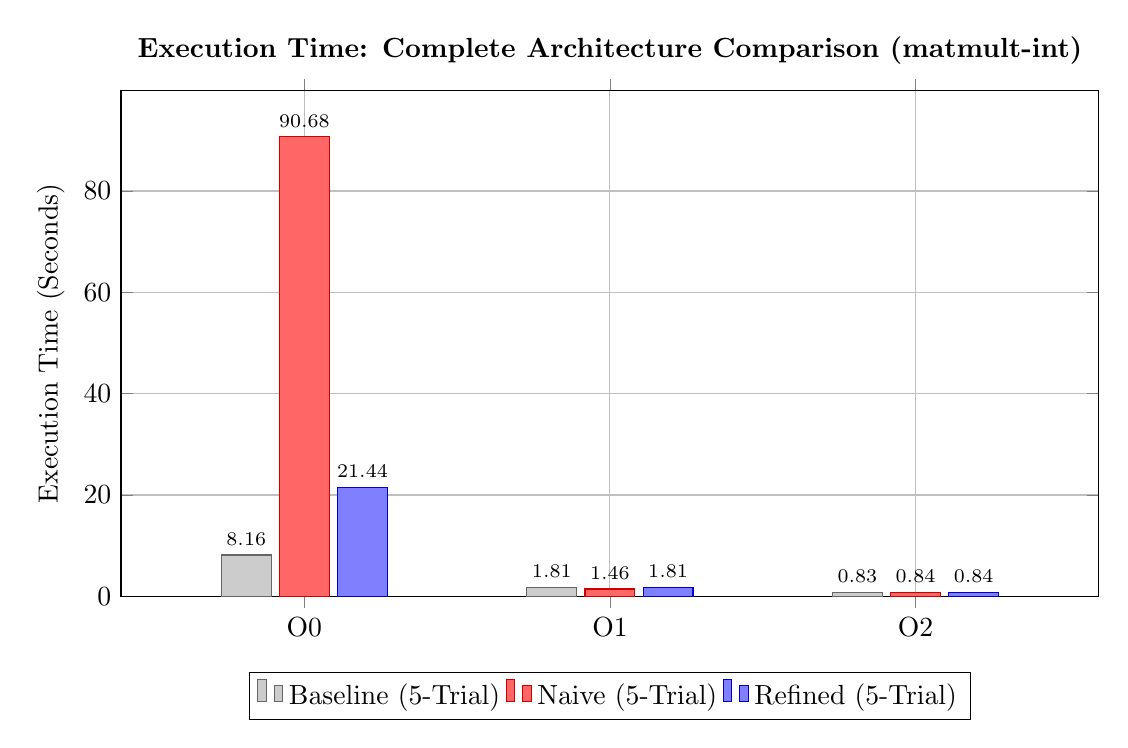
\begin{tikzpicture}
\begin{axis}[
    title={\textbf{Execution Time: Complete Architecture Comparison (matmult-int)}},
    ybar=3pt, enlarge x limits=0.3, ylabel={Execution Time (Seconds)},
    symbolic x coords={O0, O1, O2}, xtick=data, bar width=18pt,
    nodes near coords, every node near coord/.append style={font=\scriptsize},
    legend style={at={(0.5,-0.15)}, anchor=north, legend columns=-1},
    width=14cm, height=8cm, grid=major, ymin=0
]
\addplot[fill=gray!40, draw=gray!80!black] coordinates {(O0, 8.16) (O1, 1.81) (O2, 0.83)};
\addplot[fill=red!60, draw=red!80!black] coordinates {(O0, 90.68) (O1, 1.46) (O2, 0.84)};
\addplot[fill=blue!50, draw=blue!80!black] coordinates {(O0, 21.44) (O1, 1.81) (O2, 0.84)};
\legend{Baseline (5-Trial), Naive (5-Trial), Refined (5-Trial)}
\end{axis}
\end{tikzpicture}
\end{document}
